\documentclass[12pt,a4paper]{article}
\usepackage{tikz}
\begin{document}
	\begin{enumerate}
		\item 
			\begin{itemize}
				\item[(a)] The minimum value of K that may cause the system deadlock is $4$. Since we have $8$ printers and each of the processes can take no more than $3$ printers, if $K=3$, then even the $3$ processses require $3$ printer at the same time, we can always satisfy two of them first, then the two process will finish after a certain time and give back their resources and then we can satisfy the third one. However, if $K=4$, when all $4$ processes have taken $2$ printers and are requiring for one more printer, then the four conditions that will cause a deadlock are all satisfied, and there will be a deadlock.
				
				\item[(b)] No. The reason is that, no matter how big $K$ is, there is a possibility that all the processes just need one or two printers, and in such a case, we can find a safe sequence, thus the system is in safe sate and there will be no deadlock. 
			\end{itemize}
		
		\item
			\begin{itemize}
				\item[(a)]  From the table we know that\\
				\begin{minipage}{0.45\textwidth}
					\centering
					\begin{displaymath}
					\mathbf{MAX} =
					\left( \begin{array}{cccc}
					0 & 0 & 1 & 2 \\
					2 & 7 & 5 & 0 \\
					6 & 6 & 5 & 6 \\
					4 & 3 & 5 & 6 \\
					0 & 6 & 5 & 2 \\
					\end{array} \right)
					\end{displaymath}
				\end{minipage}
				\hspace{5mm}
				\begin{minipage}{0.45\textwidth}
					\centering
					\begin{displaymath}
					\mathbf{Allocation} =
					\left( \begin{array}{cccc}
					0 & 0 & 1 & 2 \\
					2 & 0 & 0 & 0 \\
					0 & 0 & 3 & 4 \\
					2 & 3 & 5 & 4 \\
					0 & 3 & 3 & 2 \\
					\end{array} \right)
					\end{displaymath}
				\end{minipage}
			Since $\mathbf{Need} = \mathbf{MAX} - \mathbf{Allocation}$, we have 
			\begin{displaymath}
			\mathbf{Need} =
			\left( \begin{array}{cccc}
			0 & 0 & 0 & 0 \\
			0 & 7 & 5 & 0 \\
			6 & 6 & 2 & 2 \\
			2 & 0 & 0 & 2 \\
			0 & 3 & 2 & 0 \\
			\end{array} \right)
			\end{displaymath}
			
			\item[(b)] Yes. Because we can find a safe sequence by banker's algorithm, that is, $P_0, P_3, P_4, P_1, P_2$.
			
			\item[(c)] We know that $\mathbf{Request_2} = (0,2,0,0)$ and $\mathbf{Available} = (2,1,0,0)$.Since $\mathbf{Request_2} \leq \mathbf{Need_2}$, but $\mathbf{Request_2} \not\leq \mathbf{Available}$, thus $P_2$ has to wait until the resources are available.
			\end{itemize}
		
		\item
			\begin{itemize}
				\item[(a)] 
					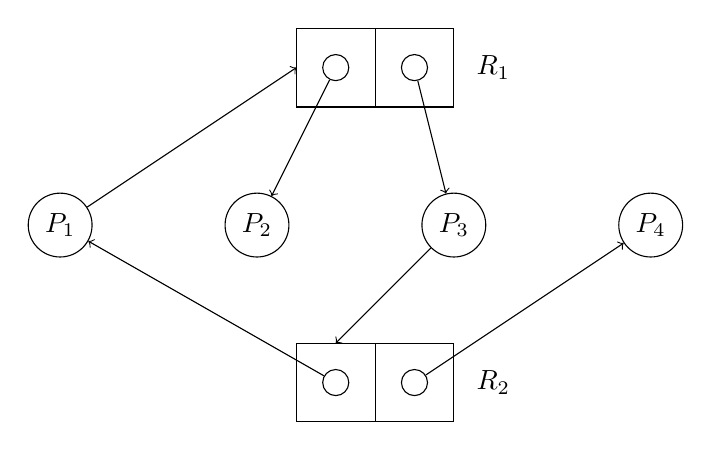
\begin{tikzpicture}
					\path (5.5,2) node (R1) {$R_1$};
					\path (5.5,-2) node (R2) {$R_2$};
					\tikzstyle{every node}=[draw,shape=circle];
						\draw (3,1.5) rectangle (4,2.5);
						\draw (4,1.5) rectangle (5,2.5);
						\draw (3,-1.5) rectangle (4,-2.5);
						\draw (4,-1.5) rectangle (5,-2.5);
						\path (0,0) node (P1) {$P_1$};
						\path (2.5,0) node (P2) {$P_2$};
						\path (5,0) node (P3) {$P_3$};
						\path (7.5,0) node (P4) {$P_4$};
						\path (3.5,2) node (r11) {};
						\path (4.5,2) node (r12) {};
						\path (3.5,-2) node (r21) {};
						\path (4.5,-2) node (r22) {};
						\draw[->] (r11) -- (P2);
						\draw[->] (r12) -- (P3);
						\draw[->] (r22) -- (P4);
						\draw[->] (r21) -- (P1);
						\draw[->] (P1) -- (3,2);
						\draw[->] (P3) -- (3.5,-1.5);
					\end{tikzpicture}
				\item[(b)] Yes. The cycle is $P_1 \rightarrow R_1 \rightarrow P_3 \rightarrow R_2 \rightarrow P_1$. We can name it $C_{P_1,P_3}$.
				
				\item[(c)] No. A possible sequence of executions is $P_2,P_4,P_1,P_3$.
			\end{itemize}
		
		\item From the table we know that\\
		\begin{minipage}{0.45\textwidth}
			\centering
			\begin{displaymath}
			\mathbf{MAX} =
			\left( \begin{array}{ccccc}
			1 & 1 & 2 & 1 & 3 \\
			2 & 2 & 2 & 1 & 0 \\
			2 & 1 & 3 & 1 & 0 \\
			1 & 1 & 2 & 2 & 1 \\
			\end{array} \right)
			\end{displaymath}
		\end{minipage}
		\hspace{5mm}
		\begin{minipage}{0.45\textwidth}
			\centering
			\begin{displaymath}
			\mathbf{Allocation} =
			\left( \begin{array}{ccccc}
			1 & 0 & 2 & 1 & 1 \\
			2 & 0 & 1 & 1 & 0 \\
			1 & 1 & 0 & 1 & 0 \\
			1 & 1 & 1 & 1 & 0 \\
			\end{array} \right)
			\end{displaymath}
		\end{minipage}
		Since $\mathbf{Need} = \mathbf{MAX} - \mathbf{Allocation}$, we have 
		\begin{displaymath}
		\mathbf{Need} =
		\left( \begin{array}{ccccc}
		0 & 1 & 0 & 0 & 2 \\
		0 & 2 & 1 & 0 & 0 \\
		1 & 0 & 3 & 0 & 0 \\
		0 & 0 & 1 & 1 & 1 \\
		\end{array} \right)
		\end{displaymath}
		By comparing $\mathbf{Need_i}$, where $i \in \{1,2,3,4\}$ with $\mathbf{Available}$, we know that if we want the system in a safe state, then $X \geq 1$. Let $X = 1$, we can find a safe sequence, that is, $D,A,C,B$. Thus, the smallest value of $X$ for which the system is in a safe state is $1$.
	\end{enumerate}
\end{document}